\documentclass[border=5pt]{standalone}
\usepackage{fourier}
\usepackage{tkz-euclide}
\begin{document}
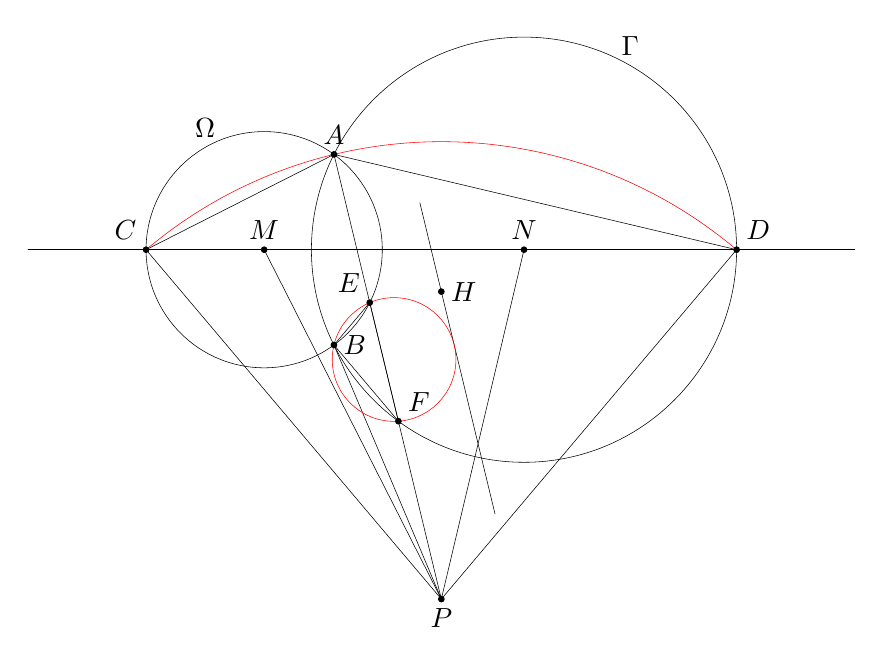
\begin{tikzpicture}
  \tkzDefPoints{0/0/C,1.5/0/M,4.8/0/N,7.5/0/D}
  \tkzInterCC(M,C)(N,D)\tkzGetPoints{A}{B}
	\tkzDefTriangleCenter[circum](A,C,D)\tkzGetPoint{P}
	\tkzDefTriangleCenter[ortho](P,M,N)\tkzGetPoint{H}
	\tkzInterLC(A,P)(M,C)\tkzGetPoints{E}{E'}
	\tkzInterLC(A,P)(N,D)\tkzGetPoints{F'}{F}
	\tkzDefTriangleCenter[circum](B,E,F)\tkzGetPoint{G}
	\tkzDefLine[parallel=through H](A,P)\tkzGetPoint{H'}
  \tkzDrawLine[add =0.2 and -0.5](H,H')
	\tkzDrawPolygon(A,C,D)
	\tkzDrawPolygon(P,M,N)
	\tkzDrawPolygon(B,E,F)
	\tkzDrawLine(C,D)
	\tkzDrawArc[red](P,D)(C)
	\tkzDrawSegments(P,A P,B P,C P,D)
	\tkzDrawCircle[black](M,C)
	\tkzDrawCircle[black](N,D)
	\tkzDrawCircle[red](G,B)
	\tkzDrawPoints[fill=black](A,B,C,M,N,D,H,E,F,P)
	\tkzLabelPoints[above](A,M,N)
	\tkzLabelPoints[above left](C,E)
	\tkzLabelPoints[right](H,B)
	\tkzLabelPoints[above right](D,F)
	\tkzLabelPoints(P)
	\tkzLabelCircle[above](M,C)(-60){$\Omega$}
	\tkzLabelCircle[above](N,D)(60){$\Gamma$}
\end{tikzpicture}
\end{document}